%%%%%%%%%%%%%%%%%%%%%%%%%%%%%%%%%%%%%%%%%%%%%%%%%%%%%%%%%%%%%%%%%%%%%%%%%%%%%%%%%%%%%%%%%%%%%%%%%%%%
% ==================================================================================================
% --------------------------------------------------------------------------------------------------
\chapter{Additional Results}
This section presents various results which are not essential to the thesis.
%%%%%%%%%%%%%%%%%%%%%%%%%%%%%%%%%%%%%%%%%%%%%%%%%%%%%%%%%%%%%%%%%%%%%%%%%%%%%%%%%%%%%%%%%%%%%%%%%%%%
\section{FLAIR MRI Intensity Modelling}\label{s:simflair}
While MR imaging is both complex and mutable,
simulation of the expected signal intensities is possible
using the relaxometry data in Table~\ref{tab:t1t2tissues} and
sequence signal equations -- e.g.\ (\ref{eq:MRI-SE}) and (\ref{eq:MRI-IR}).
In practice, this simulation helps select appropriate acquisition parameters $TE/TR/TI$
for the desired contrast;
however, these characteristics can also be later considered
as covariates in performance analysis of segmentation tools.
To this end, Equations (\ref{eq:MRI-SE}) and (\ref{eq:MRI-IR})
were used with the relaxometry data from Table~\ref{tab:t1t2tissues}
to calculate expected tissue intensities and $WMH$ contrasts.
Nine sets of acquisition parameters were taken from
the FLAIR image database (Table~\ref{tab:database}),
in addition to one simulated T1 image (TE/TR = 5/15 ms)
and one simulated T2 image (TE/TR = 100/5500 ms).
These results are summarized in Table~\ref{tab:simflair}.
In Figure~\ref{fig:simflair}, an example image is shown for each parameter set
using the tissue maps from the BrainWeb database~\cite{Collins1998},%
\footnote{\hreftt{http://brainweb.bic.mni.mcgill.ca/}}
while in Figure~\ref{fig:simflairplot},
the PMF for each tissue class from the same data are given.
\begin{table}
  \centering
  \caption{Simulated FLAIR tissue intensities and WMH contrasts
    using scan parameters from the experimental database.
    Tissue intensities are normalized to the WM value.}%
  \label{tab:simflair}
  \begin{tabular}{rccccccc}
\toprule
Scanner & \gm{} & \wm{} & \csf{} & \wmh{} & $\frac{\wmh}{\gm}$ & $\frac{\wmh}{\wm}$ & $\frac{\wmh}{\csf}$ \\
\midrule
WMH 2017 (1) & 1.21 & 1.00 & 0.26 & 1.67 & 1.38 & 1.67 & 6.32 \\
WMH 2017 (2) & 1.11 & 1.00 & 0.05 & 1.28 & 1.16 & 1.28 & 25.29 \\
WMH 2017 (3) & 1.14 & 1.00 & 0.01 & 1.49 & 1.31 & 1.49 & 105.74 \\
MS  2016 (1) & 1.32 & 1.00 & 0.00 & 3.40 & 2.57 & 3.40 & $\infty$ \\
MS  2016 (2) & 1.28 & 1.00 & 0.00 & 3.05 & 2.38 & 3.05 & $\infty$ \\
MS  2016 (3) & 1.38 & 1.00 & 0.08 & 4.08 & 2.96 & 4.08 & 48.09 \\
MS  2008 UNC & 1.21 & 1.00 & 0.53 & 1.67 & 1.38 & 1.67 & 3.17 \\
ISBI MS 2015 & 1.13 & 1.00 & 0.29 & 1.30 & 1.15 & 1.30 & 4.51 \\
In-House & 1.21 & 1.00 & 0.53 & 1.67 & 1.38 & 1.67 & 3.17 \\
T1 e.g. & 0.68 & 1.00 & 0.21 & 0.54 & 0.79 & 0.54 & 2.50 \\
T2 e.g. & 1.29 & 1.00 & 3.25 & 1.89 & 1.47 & 1.89 & 0.58 \\
\bottomrule
\end{tabular}
\end{table}
\begin{figure}
  \centering
  \foreach \i/\iname in {% % chktex 1
    01/WMH 2017 (1),
    02/WMH 2017 (2),
    03/WMH 2017 (3),
    04/MS  2016 (1),
    05/MS  2016 (2),
    06/MS  2016 (3),
    08/MS  2008 UNC,
    09/ISBI MS 2015,
    10/In-House}{%
    \begin{subfigure}{0.25\textwidth}%
      \centering\includegraphics[width=\textwidth]{simflair-s=\i.png}%
      \caption{\iname}%
    \end{subfigure}
  }\\[0.5em]
  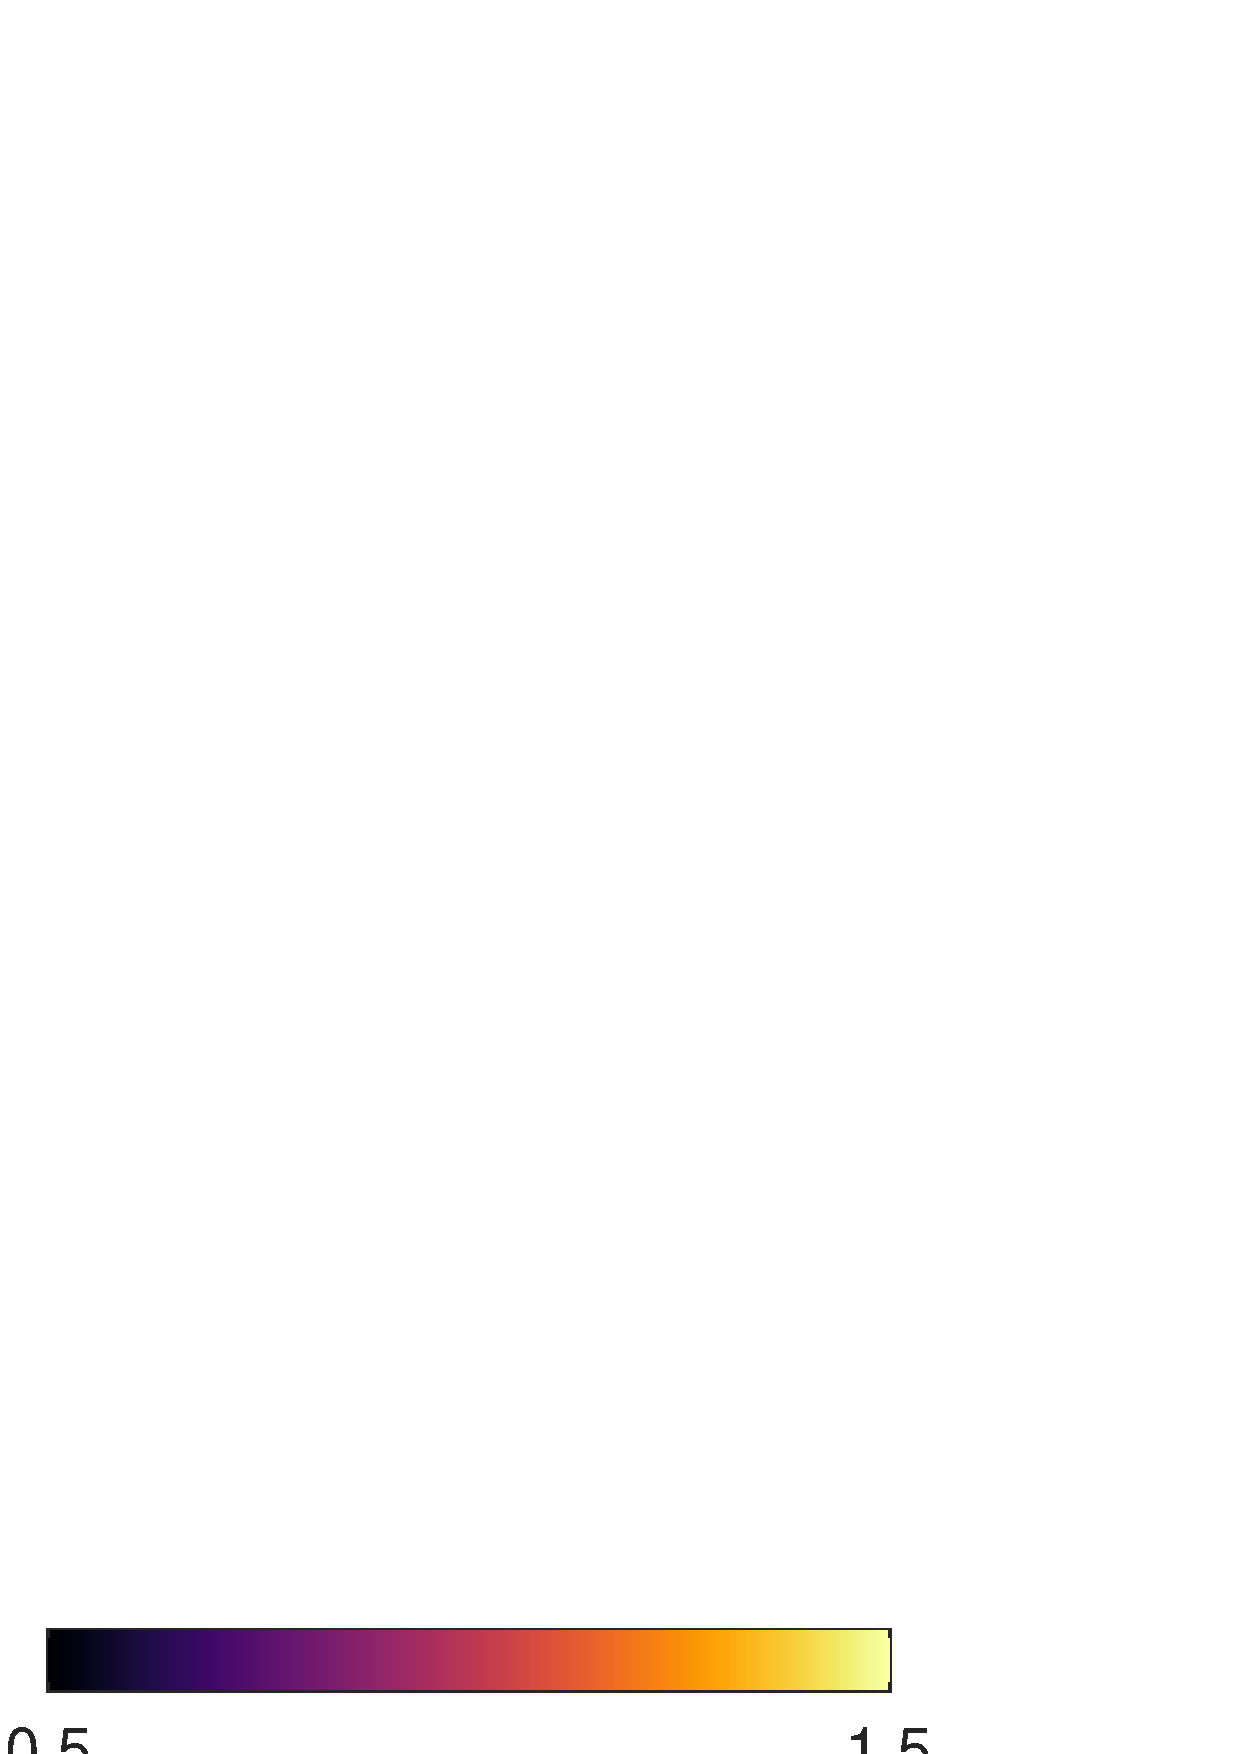
\includegraphics[width=0.25\textwidth]{hcbar-simflair}
  \caption{Simulated FLAIR images using scan parameters from the experimental database.
    Colourmap is arbitrary but consistent. Best viewed in colour.}%
  \label{fig:simflair}
\end{figure}
\begin{figure}
  \centering
  \begin{subfigure}{0.25\textwidth}
    \centering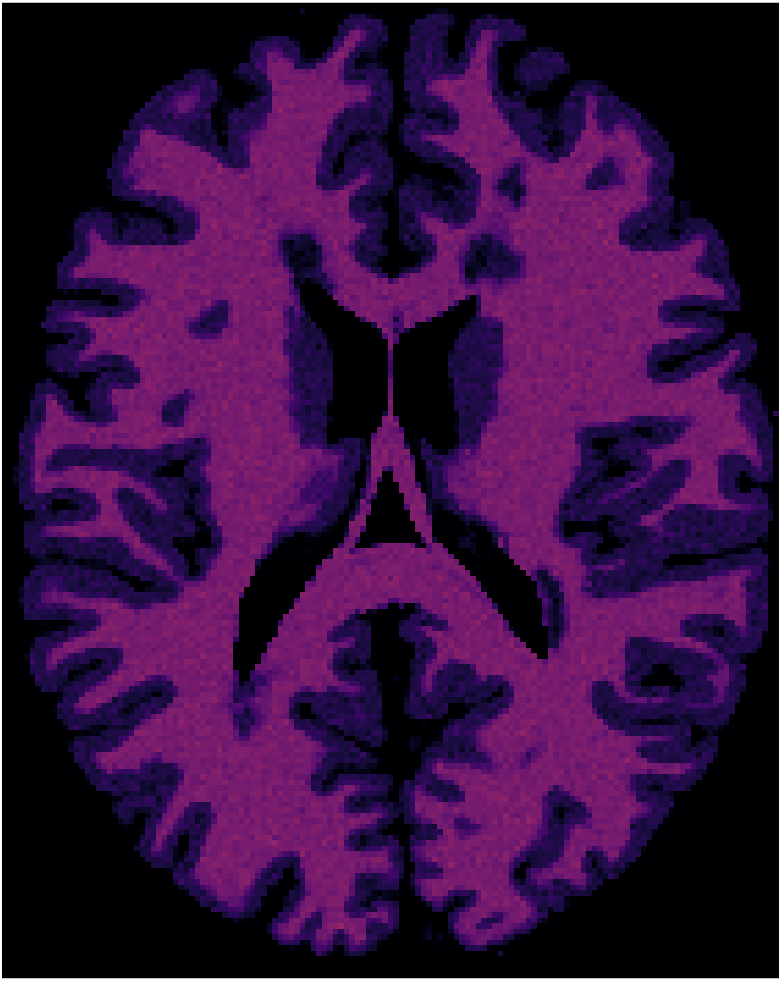
\includegraphics[width=\textwidth]{simflair-s=11.png}%
    \caption{T1}
  \end{subfigure}
  \begin{subfigure}{0.25\textwidth}
    \centering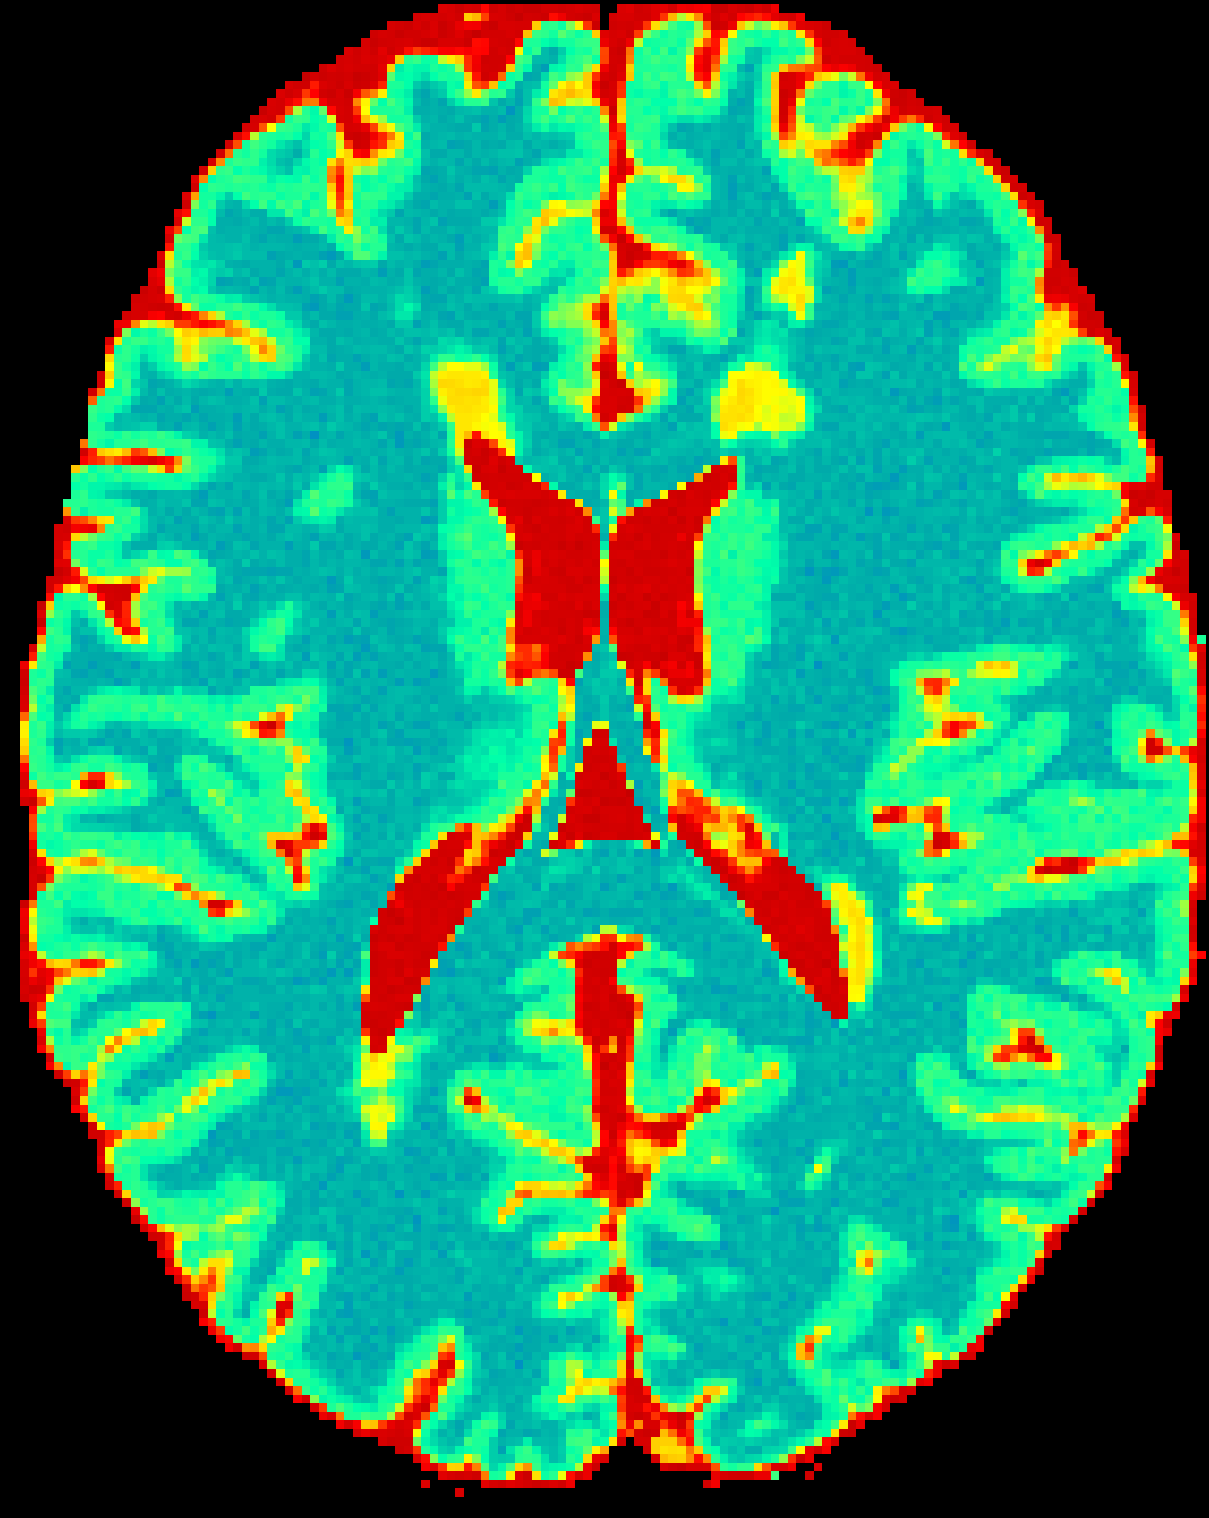
\includegraphics[width=\textwidth]{simflair-s=12.png}%
    \caption{T2}
  \end{subfigure}
  \caption{Simulated T1 (TE/TR = 5/15 ms) and T2 (TE/TR = 100/5500 ms) images.
  Best viewed in colour.}%
  \label{fig:simt1t2}
\end{figure}
\begin{figure}
  \centering
  \foreach \i/\iname in {% % chktex 1
    01/WMH 2017 (1),
    02/WMH 2017 (2),
    03/WMH 2017 (3),
    04/MS  2016 (1),
    05/MS  2016 (2),
    06/MS  2016 (3),
    08/MS  2008 UNC,
    09/ISBI MS 2015,
    10/In-House}{%
    \begin{subfigure}{0.8\plotwidth}%
      \centering\includegraphics[width=\textwidth]{simflairplot-s=\i}%
      \caption{\iname}%
    \end{subfigure}
  }\\
  \begin{subfigure}{0.8\plotwidth}%
    \centering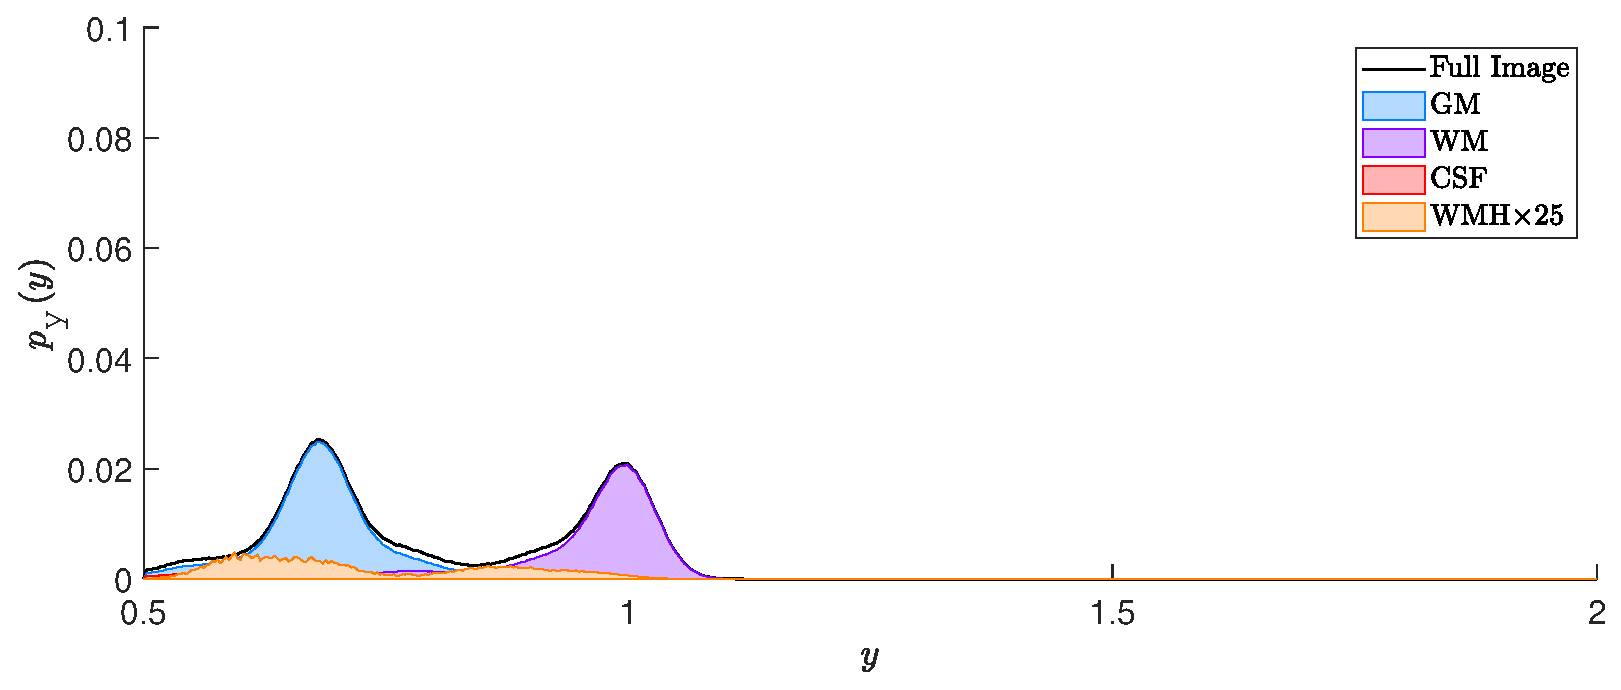
\includegraphics[width=\textwidth]{simflairplot-s=11}%
    \caption{T1 e.g.}%
  \end{subfigure}
  \begin{subfigure}{0.8\plotwidth}%
    \centering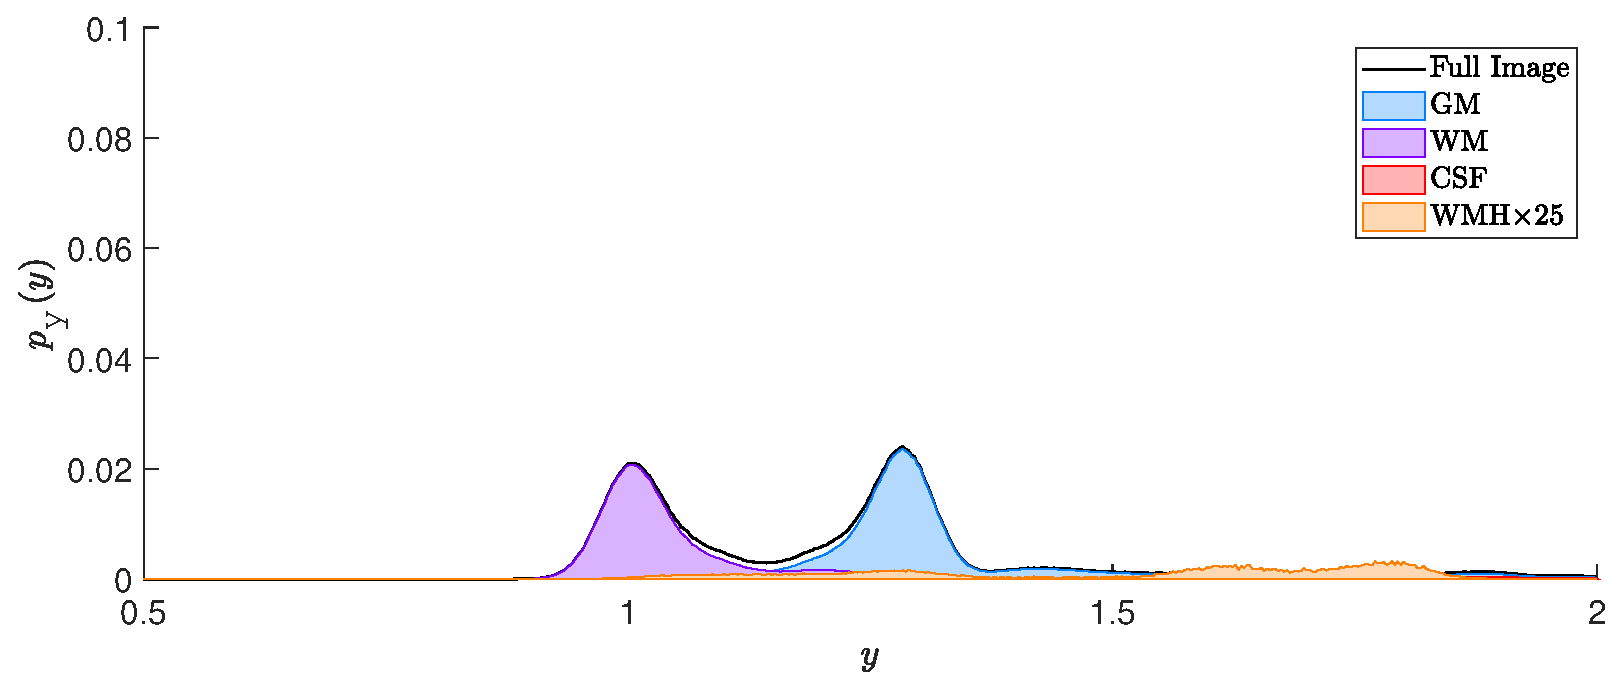
\includegraphics[width=\textwidth]{simflairplot-s=12}%
    \caption{T2 e.g.}%
  \end{subfigure}
  \caption{PMF of each tissue from simulated FLAIR, T1, and T2 images.
    The PMF of the WMH class is scaled by 25 for visibility.
    Best viewed in colour.}%
  \label{fig:simflairplot}
\end{figure}
%%%%%%%%%%%%%%%%%%%%%%%%%%%%%%%%%%%%%%%%%%%%%%%%%%%%%%%%%%%%%%%%%%%%%%%%%%%%%%%%%%%%%%%%%%%%%%%%%%%%
\section{Graylevel Standardization}
% ==================================================================================================
\subsection{Histogram Matching vs Histogram Equalization}\label{ss:hm-vs-he}
In \S~\ref{s:pre-ystd} it was argued that
histogram matching is equivalent to histogram equalization
in terms of effectiveness at standardizing graylevels in heterogeneous input images.
This is because the histogram matching operation is defined as
the function composition of the histogram equalization transform of the input image, $F_{\sy}$,
and the inverse equalization transform for the desired output histogram, ${F_{\tilde{\sy}}}^{-1}$,
\begin{equation}
  \uptau(y) = {F_{\tilde{\textsc{y}}}}^{-1}\big(F_{\sy}(y)\big).
\end{equation}
The second transformation in the cascade does not depend on $Y$,
and so it is applied equally to images.
Therefore the choice of target PMF is not important for the objective of graylevel standardization.
This result is verified experimentally using synthetic images.
Four $100\times100\times100$ images were created to have the following density functions $f_{\sy}$,
\begin{itemize}[itemsep=0pt,topsep=0pt]
  \item \parbox{2cm}{Uniform:}
  $y\sim\mathcal{U}(y_{\min}=0,y_{\max}=1)$
  \item \parbox{2cm}{Unimodal:}
  $y\sim\N(\mu=0.5,\sigma=0.08)$
  \item \parbox{2cm}{Bimodal:}
  $y\sim\big(0.5\et\N(\mu=0.3,\sigma=0.05)
            +0.5\et\N(\mu=0.7,\sigma=0.05)\big)$
  \item \parbox{2cm}{Trimodal:}
  $y\sim\big(0.3\et\N(\mu=0.25,\sigma=0.05)
            +0.4\et\N(\mu=0.5,\sigma=0.05)
            +0.3\et\N(\mu=0.75,\sigma=0.05)\big)$
\end{itemize}
All four images were then histogram-matched to each of the respective density functions,
with the aim of increasing agreement of image intensities.
This agreement can be approximated by the alignment of intensity quantiles,
since this is the target of histogram matching operations.
As shown in Figure~\ref{fig:hm-vs-he}, the quantiles agree almost perfectly in every output image,
regardless of the choice of output PMF.
\begin{figure}
  \centering
  \begin{subfigure}{\plotwidth}
    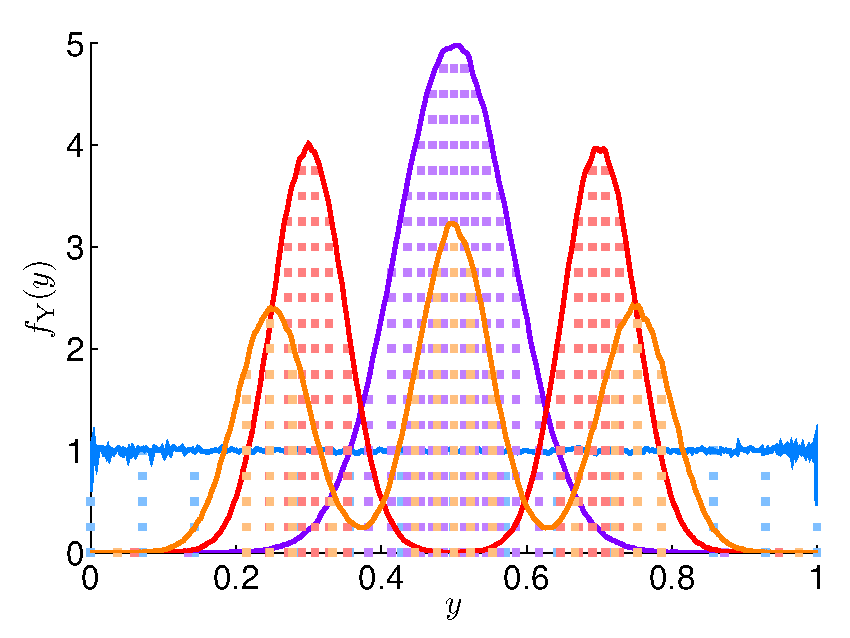
\includegraphics[width=\textwidth]{histmatch-q-original}
    \caption{Original}
  \end{subfigure}
  \parbox[c]{\plotwidth}{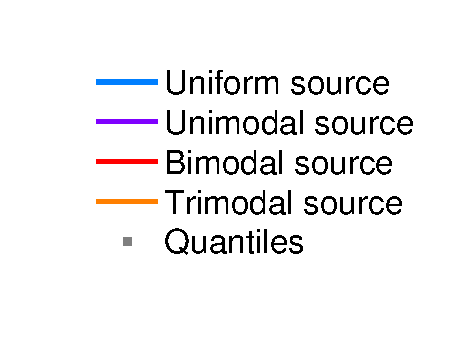
\includegraphics[width=0.7\plotwidth]{histmatch-q-legend}}\\
  \begin{subfigure}{\plotwidth}
    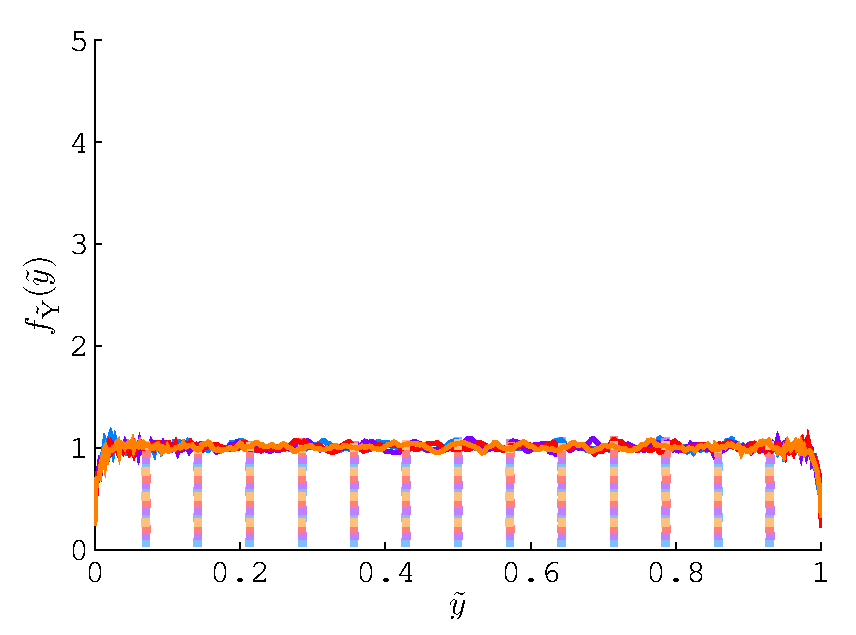
\includegraphics[width=\textwidth]{histmatch-q-uniform}
    \caption{Uniform target}
  \end{subfigure}
  \begin{subfigure}{\plotwidth}
    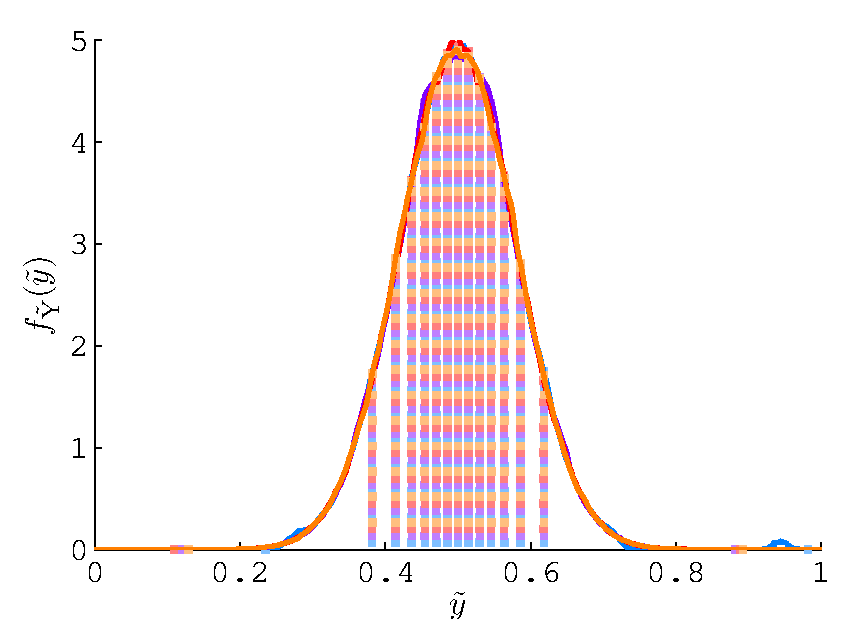
\includegraphics[width=\textwidth]{histmatch-q-unimodal}
    \caption{Unimodal target}
  \end{subfigure}
  \begin{subfigure}{\plotwidth}
    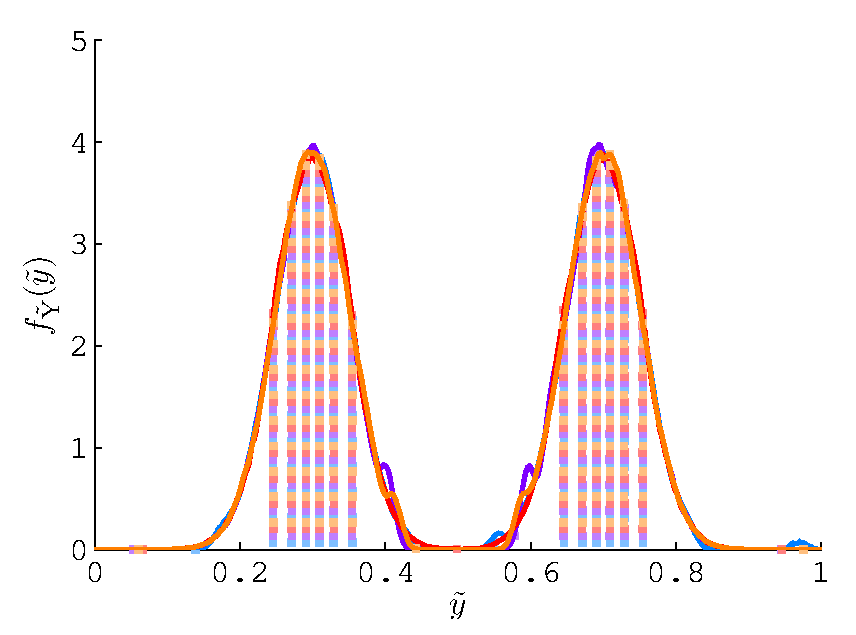
\includegraphics[width=\textwidth]{histmatch-q-bimodal}
    \caption{Bimodal target}
  \end{subfigure}
  \begin{subfigure}{\plotwidth}
    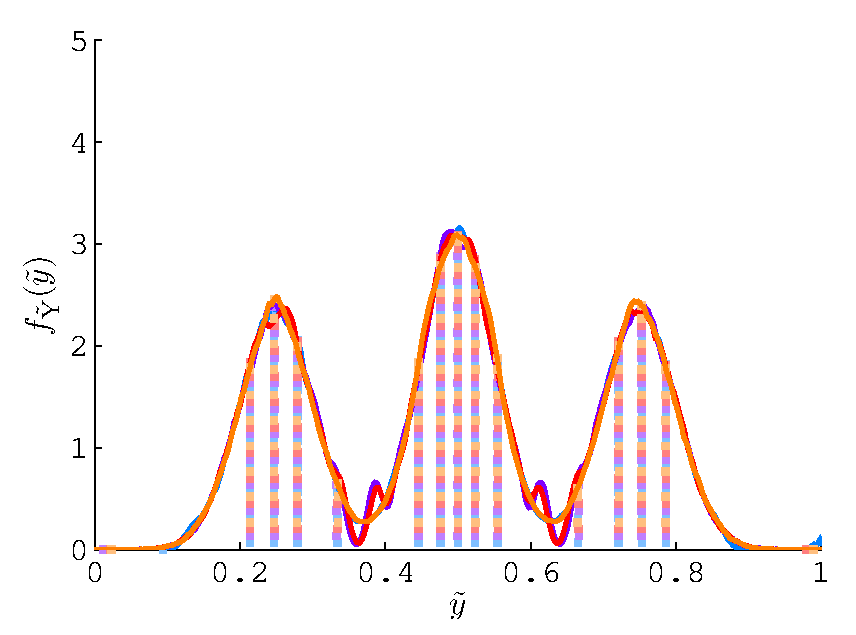
\includegraphics[width=\textwidth]{histmatch-q-trimodal}
    \caption{Trimodal target}
  \end{subfigure}
  \caption{Histogram matching of synthetic data to different target histograms.
    Quantiles show high agreement regardless of the target histogram.
    Best viewed in colour.}%
  \label{fig:hm-vs-he}
\end{figure}
\clearpage
%%%%%%%%%%%%%%%%%%%%%%%%%%%%%%%%%%%%%%%%%%%%%%%%%%%%%%%%%%%%%%%%%%%%%%%%%%%%%%%%%%%%%%%%%%%%%%%%%%%%
\section{Segmentation Performance Data}
This section presents the raw performance data for all model iterations used in the thesis,
which compare various regularization strategies and cross validation frameworks.
Median values shown throughout.
\begin{singlespace}
  \centering
  \CatchFileDef{\tablist}{./figs/tab/table-index.tex}{\endlinechar=`,}
  \edef\tablistfun{\unexpanded{\foreach\cap/\file in }{\unexpanded\expandafter{\tablist}}}% % chktex 1
  \tablistfun{\begin{minipage}{\plotwidth}%
      {\centering\cap\par\vspace{0.5em}\input{./figs/tab/\file}}\vspace{1em}% % chktex 27
  \end{minipage} }
\end{singlespace}
% --------------------------------------------------------------------------------------------------
% ==================================================================================================
%%%%%%%%%%%%%%%%%%%%%%%%%%%%%%%%%%%%%%%%%%%%%%%%%%%%%%%%%%%%%%%%%%%%%%%%%%%%%%%%%%%%%%%%%%%%%%%%%%%%
